\documentclass[12pt,letterpaper]{article}

% ── Packages ──────────────────────────────────────────────────────────────────
\usepackage[T1]{fontenc}
\usepackage[utf8]{inputenc}
\usepackage{lmodern}
\usepackage{microtype}
\usepackage{amsmath,amssymb,amsthm}
\usepackage{bm}
\usepackage{booktabs}
\usepackage{array}
\usepackage{multirow}
\usepackage{graphicx}
\usepackage{xcolor}
\usepackage{hyperref}
\usepackage{url}
% \usepackage{natbib}  % not needed with manual thebibliography
\usepackage{geometry}
\usepackage{parskip}
\usepackage{enumitem}
\usepackage{listings}
\usepackage{caption}
\usepackage{subcaption}
\usepackage{algorithm}
\usepackage{algpseudocode}
\usepackage{tikz}
\usetikzlibrary{arrows.meta,positioning,shapes.geometric,fit,backgrounds,calc}

\geometry{margin=1.1in}

\hypersetup{
  colorlinks=true,
  linkcolor=blue!60!black,
  citecolor=blue!60!black,
  urlcolor=blue!60!black,
}

\lstset{
  basicstyle=\ttfamily\small,
  breaklines=true,
  frame=single,
  backgroundcolor=\color{gray!8},
  commentstyle=\color{gray!70!black},
  keywordstyle=\color{blue!70!black},
  language=Python,
  showstringspaces=false,
}

% ── Theorem environments ───────────────────────────────────────────────────────
\newtheorem{proposition}{Proposition}
\newtheorem{definition}{Definition}

% ── Math shorthands ───────────────────────────────────────────────────────────
\newcommand{\RR}{\mathbb{R}}
\newcommand{\bF}{\mathbf{F}}
\newcommand{\bp}{\mathbf{p}}
\newcommand{\bB}{\mathbf{B}}
\newcommand{\bg}{\mathbf{g}}
\newcommand{\bx}{\mathbf{x}}
\newcommand{\bc}{\mathbf{c}}
\newcommand{\bq}{\mathbf{q}}
\newcommand{\T}{\mathsf{T}}
\newcommand{\norm}[1]{\left\lVert#1\right\rVert}
\newcommand{\inner}[2]{\langle#1,\,#2\rangle}

% ──────────────────────────────────────────────────────────────────────────────

\title{\textbf{WaveRider: A Zero-Parameter Geometric Machine Learning\\
Stack for Manifold-Aware Classification}}

\author{
  Eric G.\ Suchanek, PhD\\
  Independent Researcher\\
  \texttt{suchanek@mac.com}\\[4pt]
  \small\url{https://github.com/suchanek/proteusPy}
}

\date{March 2026}

\begin{document}

\maketitle

\begin{abstract}
We present \textbf{WaveRider}, a four-layer framework for manifold-aware machine
learning that achieves competitive classification without learned parameters.
The core thesis is that \emph{the manifold is the model}: the data manifold,
once discovered through local principal component analysis and encoded as a
weighted knowledge graph with stored basis geometry, is itself a sufficient
classifier.

WaveRider consists of: (1)~\textbf{TurtleND}, an $N$-dimensional navigation
primitive carrying position and an orthonormal frame, generalised from the
classical Turtle3D molecular modelling primitive via Givens rotations;
(2)~\textbf{ManifoldWalker} and its Adam variant, implementing
Riemannian-approximate gradient descent by projecting updates onto
locally-estimated tangent planes; (3)~\textbf{ManifoldModel}, a zero-parameter
classifier whose ``weights'' are the graph topology, local basis vectors, and
eigenvalue field discovered during a single exploration pass; and
(4)~\textbf{ManifoldObserver}, a novel $(N+1)$-dimensional construction that
extends any $N$-dimensional manifold frame by one orthonormal dimension via QR
decomposition, gaining the manifold normal and the ability to observe curvature,
topology, and class boundaries from \emph{above} the surface---turning a search
problem into a projection problem.

The ManifoldObserver operationalises a principle with deep roots: Plato's
prisoners see only shadows on the cave wall until lifted into three dimensions;
Abbott's Flatlanders see only slices until raised above their plane; Gauss's
extrinsic curvature is invisible from the surface until one dimension is added.
WaveRider provides the constructive machine-learning instantiation of this
principle.

On the UCI Digits dataset (64 dimensions) ManifoldModel achieves 97.72\%
accuracy with zero parameters versus 97.33\% for Euclidean KNN\@.
On CIFAR-10 (3{,}072 dimensions) ManifoldModel uses $219{\times}$ fewer parameters
than a standard CNN while matching its accuracy.
The ManifoldObserver achieves 100\% agreement with its $N$-dimensional subject
on synthetic benchmarks while providing curvature and topology information
unavailable to the surface-bound walker.
We also describe an application to protein disulfide bond analysis, where a
6-dimensional observer looks into the 5-dimensional torsion-angle manifold and
sees the structural landscape that the walker must search.
\end{abstract}

% ──────────────────────────────────────────────────────────────────────────────
\section{Introduction}
% ──────────────────────────────────────────────────────────────────────────────

The dominant paradigm in machine learning is to fit a parameterised function---a
neural network, a kernel machine, a decision tree---to training data by
optimising a loss. The resulting weights encode, implicitly, knowledge about the
data distribution. This works well but has a cost: millions of parameters for
complex tasks, opacity about what was learned, and fragility when the test
distribution shifts.

An alternative is to \emph{discover} the data manifold explicitly and use that
discovery as the model. Real high-dimensional data---images, protein structures,
speech signals---rarely uses all of its ambient dimensions.
Handwritten digits ($8{\times}8$ pixels) lie on a manifold of intrinsic
dimension $\approx$13 inside 64-dimensional space (71--83\% of ambient
dimensions are noise).
CIFAR-10 natural images lie on a manifold of local intrinsic dimension 23--36
inside 3{,}072-dimensional space (98.8--99.3\% noise), depending on the
variance threshold $\tau$ (Section~\ref{sec:manifoldwalker},
Table~\ref{tab:tau}).

These intrinsic dimensions are not assumed: they are \emph{discovered} by
WaveRider's local PCA estimator (Algorithm~\ref{alg:walker}, step~3).
For each data point, the $k$-nearest-neighbour covariance matrix is
diagonalised; the intrinsic dimension $d$ is the minimum number of principal
components whose cumulative eigenvalue fraction reaches $\tau$.
This per-point, data-driven estimate is consistent with independent global
measurements using the TwoNN estimator~\cite{facco17} and with prior surveys
of image-dataset intrinsic dimensionality~\cite{pope21}.

If we can find the manifold, we can discard the noise, measure distances
correctly (along the surface, not through the void), and classify by
\emph{geometry} rather than by optimisation.

WaveRider does exactly this. It is not the first work to identify the manifold
hypothesis~\cite{isomap,lle}, nor the first to use local PCA for dimensionality
reduction~\cite{kambhatla97,hinton06}. What is novel is the integration: a
coherent stack from a navigation primitive through optimisation to a
zero-parameter classifier to an $(N+1)$-dimensional extrinsic observer that can
see what the classifier cannot.

The key conceptual contributions are:

\begin{enumerate}[leftmargin=*]
\item \textbf{TurtleND}---the formal generalisation of Turtle3D to $N$
  dimensions using Givens rotations, enabling navigation in
  arbitrary-dimensional data spaces with the same primitives (move, rotate,
  orient) used for molecular modelling since 1986.

\item \textbf{ManifoldModel}---the identification that a $k$-NN graph with
  stored local PCA geometry at each node \emph{is itself} a classifier, with no
  additional learned weights.  Classification is manifold-aware nearest-neighbour
  search over this graph.

\item \textbf{ManifoldObserver}---a constructive proof that any $N$-dimensional
  manifold frame can be extended to $(N+1)$ dimensions by a single QR
  decomposition, gaining the manifold normal.  The observer classifies by
  projection rather than search, observes curvature and topology in $O(n)$
  rather than $O(\text{hops} \times k)$, and embodies the geometric principle:
  \emph{to understand a surface, you must leave it}.
\end{enumerate}

\subsection{Motivation: From Molecular Modelling to Machine Learning}

The WaveRider stack did not originate in machine learning.  It originated in
molecular modelling.  The Turtle3D class in
proteusPy~\cite{suchanek24joss} was designed to build protein structures by
navigating local coordinate frames along bond vectors---a technique dating to the
author's 1992 \emph{Proteus} program~\cite{suchanek92}.  The frame carried
heading, left, and up vectors; rotations encoded dihedral angles; molecules were
``drawn'' by a turtle navigating chemical space.

The generalisation to $N$ dimensions arose when the same navigational primitive
was needed for the 5-dimensional torsion-angle space of disulfide bonds.  But
once the $N$-dimensional turtle existed, the question became: what else can it
navigate?  The answer---data manifolds---led directly to the WaveRider stack.

This origin matters: WaveRider is not an abstraction built for machine learning.
It is a navigation primitive that turned out to be equally at home in a protein
crystal and a high-dimensional embedding space.

% ──────────────────────────────────────────────────────────────────────────────
\section{Related Work}
% ──────────────────────────────────────────────────────────────────────────────

\paragraph{Manifold learning.}
Isomap~\cite{isomap}, LLE~\cite{lle}, UMAP~\cite{umap}, and t-SNE~\cite{tsne}
are standard manifold-learning tools, but they are dimensionality-reduction
methods---they produce low-dimensional embeddings for visualisation or downstream
processing.  WaveRider does not reduce dimensions; it discovers the manifold
geometry \emph{in place} and uses it directly for classification.

\paragraph{Local PCA.}
Local linear embedding~\cite{lle} and its variants use local PCA to estimate
tangent spaces.  WaveRider's ManifoldWalker and ManifoldModel use local PCA
similarly but store the full geometry (basis, eigenvalues, intrinsic dimension)
at each node rather than producing a global embedding.

\paragraph{Riemannian optimisation.}
Methods for optimisation on Riemannian manifolds~\cite{absil09,bonnabel13}
project gradients onto tangent planes and retract back to the manifold surface.
ManifoldWalker performs approximate Riemannian gradient descent without requiring
an explicit manifold parameterisation---the tangent plane is estimated locally
at each step from the data neighbourhood.

\paragraph{Geometric deep learning.}
The field of geometric deep learning~\cite{bronstein21} argues that symmetries
and geometric structure should be built into neural architectures.  WaveRider
takes this further: rather than embedding geometric structure in a \emph{trained}
model, the geometry \emph{is} the model.

\paragraph{Prototype-based classifiers.}
Learning Vector Quantisation (LVQ)~\cite{kohonen90} and its successors classify
by distance to learned prototypes.  ManifoldModel is in the spirit of
prototype-based classifiers, but the prototypes are all training points (not a
learned subset), and distances are measured in manifold space rather than
Euclidean space.

\paragraph{Intrinsic dimensionality estimation.}
Several estimators have been proposed for the intrinsic dimensionality of a
dataset.  The TwoNN estimator~\cite{facco17} derives a maximum-likelihood
estimate from the ratio of each point's first- and second-nearest-neighbour
distances under a Poisson process model on the manifold; it requires only three
nearest neighbours per point and is implemented in
\texttt{benchmarks/pepys\_manifold\_explorer.py} for global corroboration.
The participation ratio~\cite{pope21}, $\mathrm{PR} = (\sum\lambda_i)^2 /
\sum\lambda_i^2$, measures the effective number of active principal components.
PCA-based elbow methods~\cite{kambhatla97} count components up to a cumulative
variance threshold.  WaveRider uses the last of these \emph{locally} at every
graph node (Algorithm~\ref{alg:walker}, step~3), producing a per-point intrinsic
dimension field rather than a single global estimate.

\paragraph{Extrinsic vs.\ intrinsic geometry.}
The distinction between intrinsic (Gauss) curvature and extrinsic (mean
curvature, normal vectors) differential geometry is classical~\cite{docarmo76}.
The ManifoldObserver operationalises this distinction: by adding one dimension it
gains access to the manifold normal and all extrinsic quantities that are
invisible from the surface.

% ──────────────────────────────────────────────────────────────────────────────
\section{The WaveRider Stack}
% ──────────────────────────────────────────────────────────────────────────────

%% ── Figure 1: WaveRider stack schematic ──────────────────────────────────────
\begin{figure}[t]
\centering
\includegraphics[width=\linewidth]{waverider_approach.png}
\caption{The WaveRider four-layer hierarchy.  Layer~1 (\textbf{TurtleND})
provides the $N$-dimensional navigation primitive with position and orthonormal
frame; Layer~2 (\textbf{ManifoldWalker}/ManifoldAdamWalker) performs
Riemannian-approximate gradient descent via local PCA and manifold-projected
updates; Layer~3 (\textbf{ManifoldModel}/ManifoldObserver) stores the explored
geometry as a zero-parameter classifier and extends the frame by one QR step to
gain an extrinsic view of curvature, topology, and class boundaries; Layer~4
(\textbf{GraphReasoner}) performs geometry-steered reasoning over the resulting
knowledge graph.  The inset table (lower right) summarises the role of each
layer.}
\label{fig:stack}
\end{figure}
%% ─────────────────────────────────────────────────────────────────────────────

\subsection{Layer 1: TurtleND --- Navigation Primitive}

A TurtleND in $N$-dimensional space carries:
\begin{itemize}[leftmargin=*]
  \item \textbf{Position} $\bp \in \RR^N$
  \item \textbf{Frame} $\bF \in \RR^{N \times N}$, $\bF\bF^\T = I_N$ (rows are
    orthonormal basis vectors).  $\bF[0]$~=~heading, $\bF[1]$~=~left,
    $\bF[2]$~=~up, $\bF[3\ldots N{-}1]$~=~higher dimensions.
\end{itemize}

The state evolves via:

\textbf{Translation.}
$\texttt{move}(d)$: $\bp \leftarrow \bp + d\cdot\bF[0]$.

\textbf{Givens rotation} in the $(i,j)$ plane ($\theta \in \RR$):
\begin{align}
  \bF[i] &\leftarrow \cos\theta\;\bF[i] + \sin\theta\;\bF[j], \notag\\
  \bF[j] &\leftarrow -\sin\theta\;\bF[i] + \cos\theta\;\bF[j]. \label{eq:givens}
\end{align}
Named special cases: $\texttt{turn}(\theta) = R(\theta,0,1)$, $\texttt{pitch}(\theta) = R(\theta,0,2)$, $\texttt{roll}(\theta) = R(\theta,1,2)$.

\begin{proposition}[Frame Invariance]
Givens rotations in any $(i,j)$ plane preserve the orthonormality of the full
$N$-dimensional frame.
\end{proposition}
\begin{proof}
A Givens rotation is an orthogonal transformation; the product of orthogonal
matrices is orthogonal.
\end{proof}

Re-normalisation via QR recovers numerical orthonormality after
accumulated floating-point drift.  Coordinate transforms:
$\texttt{to\_local}(\mathbf{v}) = \bF\mathbf{v}$ and
$\texttt{to\_global}(\mathbf{v}) = \bF^\T\mathbf{v}$.
Turtle3D (Roll, Pitch, Yaw, Turn, Move) is the special case $N=3$.

\subsection{Layer 2: ManifoldWalker --- Gradient Descent on the Manifold}
\label{sec:manifoldwalker}

ManifoldWalker performs optimisation on an implicit manifold defined by a point
cloud, using local PCA to estimate the tangent space at each step.

\begin{algorithm}[h]
\caption{ManifoldWalker single step}
\label{alg:walker}
\begin{algorithmic}[1]
\Require current position $\bp$, loss gradient $\nabla L(\bp)$,
         dataset $\mathcal{X}$, parameters $k,\tau,\eta$
\State Find $k$ nearest neighbours of $\bp$ in $\mathcal{X}$
\State Compute neighbourhood covariance; SVD $\to$ eigenvalues
       $\bm\lambda \in \RR^N$, eigenvectors $V \in \RR^{N\times N}$
\State $d \leftarrow \min j$ s.t.\
       $\frac{\sum_{i\le j}\lambda_i}{\sum_i\lambda_i} \ge \tau$
       \quad\Comment{intrinsic dimension}
\State Orient frame $\bF$ to columns of $V$ (descending $\lambda$ order)
\State $\tilde{\bg} \leftarrow \bF^\T\nabla L(\bp)$;
       zero components $d{+}1\ldots N$ \quad\Comment{project onto manifold}
\State $\bp \leftarrow \bp - \eta\cdot\bF\tilde{\bg}$
\end{algorithmic}
\end{algorithm}

%% ── Figure 2: WaveRider algorithm architecture ────────────────────────────────
\begin{figure}[h]
\centering
\includegraphics[width=\linewidth]{waverider_arch.png}
\caption{WaveRider algorithm architecture.  Phase~1 (\textbf{Gradient Diversity
Sampling}) draws a diverse batch of gradients $g_1,\ldots,g_s$ from the current
weights.  Phase~2 (\textbf{Manifold Discovery via PCA}) computes the gradient
covariance $C = G^\mathsf{T}G/(S-1)$, diagonalises it via SVD, and selects the
top-$d$ eigenvectors; intrinsic dimension $d \approx 2$--$3$ is discovered
automatically against the ambient 243-dimensional gradient space.  Phase~3
(\textbf{Manifold Gate}) projects the full gradient onto the $d$-dimensional
signal subspace ($\mathbf{g}_\text{proj}$), suppressing 99\% of ambient noise.
Phase~4 (\textbf{ManifoldAdamWalker}) runs standard Adam momentum and adaptive
learning-rate updates on the projected gradient, re-orienting the PCA basis
every $R$ epochs.  Standard Adam tracks all 243 noisy dimensions; WaveRider
tracks only the 2--3 signal dimensions.}
\label{fig:arch}
\end{figure}
%% ─────────────────────────────────────────────────────────────────────────────

\paragraph{ManifoldAdamWalker.}
Replaces step~6 with Adam momentum~\cite{adam}:
\begin{align}
  \mathbf{m} &\leftarrow \beta_1\mathbf{m} + (1-\beta_1)\bg_\text{proj},\notag\\
  \mathbf{v} &\leftarrow \beta_2\mathbf{v} + (1-\beta_2)\bg_\text{proj}^2,\notag\\
  \bp &\leftarrow \bp - \eta\,\hat{\mathbf{m}}\,/\,(\sqrt{\hat{\mathbf{v}}}+\varepsilon),
  \label{eq:adam}
\end{align}
where $\hat{\mathbf{m}},\hat{\mathbf{v}}$ are bias-corrected estimates and
$\bg_\text{proj}$ is the manifold-projected gradient \emph{in global
coordinates}.  Keeping the Adam state in global coordinates is a critical
design decision: momentum persists across frame re-orientations as the manifold
curves, while the manifold projection ensures momentum cannot drift into
off-manifold directions.

Default parameters: $k{=}50$, $\tau{=}0.95$, $\eta{=}0.01$,
$\beta_1{=}0.9$, $\beta_2{=}0.999$, $\varepsilon{=}10^{-7}$.

\subsection{Layer 3: ManifoldModel --- The Manifold as the Classifier}

ManifoldModel operationalises the thesis: \emph{the manifold is the model}.
There are no learned weights; the trained model is the graph.

\subsubsection{Phase 1 --- Explore (Fit)}

For each training point $\bx_i$ with label $y_i$:
\begin{enumerate}[leftmargin=*]
  \item Add $(\bx_i, y_i)$ as a graph node.
  \item Compute local PCA via SVD on $k_\text{pca}$-neighbourhood covariance.
  \item Store \textbf{NodeGeometry}: truncated basis $\bB_i \in \RR^{d\times N}$,
    eigenvalues $\bm\lambda_i$, intrinsic dimension $d_i$, centroid
    $\bc_i$, label $y_i$.
\end{enumerate}

Build manifold-aware edges from node $i$ to its $k_\text{graph}$ Euclidean
nearest neighbours~$j$:
\begin{align}
  \text{manifold\_dist}_{ij} &= \norm{\bB_i(\bx_j - \bc_i)}, \label{eq:mdist}\\
  \text{dist\_blend}_{ij}    &= w\cdot\text{manifold\_dist}_{ij}
                                + (1-w)\cdot\norm{\bx_j-\bx_i}, \label{eq:blend}\\
  \text{weight}_{ij}         &= \frac{1}{1 + \text{dist\_blend}_{ij}},
  \label{eq:eweight}
\end{align}
where $w = \texttt{manifold\_weight}$ (default $0.8$).

\paragraph{The blending function (Eq.~\ref{eq:blend}).}
The convex combination in Eq.~\eqref{eq:blend} balances two failure modes.
\emph{Pure manifold distance} ($w{=}1$) measures displacement only in the local
tangent plane and cannot distinguish two points that lie in the same plane but
are far apart in ambient space; it is also degenerate in sparse neighbourhoods
where the PCA basis is under-determined.  \emph{Pure Euclidean distance}
($w{=}0$) ignores manifold structure and may connect points that are
Euclidean-close but lie on different folds of the surface.

The default $w{=}0.8$ reflects three considerations:
\begin{enumerate}[leftmargin=*,label=(\arabic*)]
  \item \textbf{Primacy of geometry}: the tangent-plane projection captures the
    directions of real signal and should dominate.
  \item \textbf{Numerical grounding}: a 20\% Euclidean component prevents
    degenerate edges at boundaries and ensures connectivity even when manifold
    distances are poorly estimated.
  \item \textbf{Empirical stability}: $\tau$-sweep benchmarks on CIFAR-10
    (Table~\ref{tab:tau}) show that accuracy is more sensitive to $\tau$ than to
    $w$ in the range $w \in [0.7, 0.9]$; the default sits at the flat centre of
    this range.
\end{enumerate}
The edge weight formula~\eqref{eq:eweight} maps blended distance to $(0,1]$
monotonically.  It is scale-invariant in the sense that the relative ordering of
edge weights is preserved under uniform scaling of the data.

\paragraph{Parameter rationale.}
$k_\text{pca}{=}50$ provides enough neighbours for stable local PCA
(rule of thumb: $k \ge 5d$; with $d \le 10$ typical, $k{=}50$ is
conservative).  $k_\text{graph}{=}15$ controls connectivity without diluting
manifold-awareness with distant nodes.  $k_\text{vote}{=}7$ is the standard odd-$k$
for majority voting.  $\tau{=}0.95$ retains 95\% of local variance;
Table~\ref{tab:tau} shows that $\tau \in \{0.85, 0.90, 0.95\}$ produces
consistent results.

\paragraph{What is stored = what is learned.}
The ``trained'' ManifoldModel consists entirely of: graph connectivity
(topology), local basis $\bB_i$ at each node (geometry), eigenvalues
$\bm\lambda_i$ (scale), and node labels (supervision).  No gradient-updated
scalars exist.

\subsubsection{Phase 2 --- Navigate (Predict)}

To classify query point $\bq$:
\begin{enumerate}[leftmargin=*]
  \item Find $k_\text{pca}$ Euclidean nearest neighbours.
  \item Compute local PCA \emph{at $\bq$} via SVD $\to$ query tangent space
    $\bB_q$.
  \item Project $\bq$ and candidates into $\bB_q$.
  \item Walk graph from nearest node (2~hops) to gather additional candidates.
  \item Distance-weighted majority vote among $k_\text{vote}$ nearest in
    projected space.
\end{enumerate}
Cost: $O(k_\text{pca} N)$ local PCA $+$ $O(k_\text{graph}^2)$ graph walk $+$
$O(k_\text{vote})$ vote.

\subsubsection{Phase 3 --- Fly (Interactive Exploration)}

The fitted ManifoldModel supports interactive navigation: \texttt{fly\_to},
\texttt{fly\_step}, and \texttt{fly\_toward} allow a user (or agent) to enter
the manifold at any point and explore by heading toward regions of interest, with
the frame always re-aligning to local geometry at each hop.  This \emph{fly
mode} provides a form of knowledge navigation unavailable in standard
classifiers.

\subsection{Layer 3a: ManifoldObserver --- Extrinsic Observer}
\label{sec:observer}

The ManifoldObserver is the central novel contribution of this work.
It gives an extrinsic viewpoint into the $N$-dimensional data manifold from
$(N+1)$-dimensional space.

\subsubsection{The Construction}

Given the ManifoldModel's subject turtle at a manifold node with $N$-dimensional
orthonormal frame $\bF \in \RR^{N \times N}$:

\textbf{Step 1: Pad.}  Extend each row of $\bF$ with a zero in position $N$;
append row $\mathbf{e}_N = [0,\ldots,0,1] \in \RR^{N+1}$:
\[
  F_\text{ext} \in \RR^{(N+1)\times(N+1)}, \quad
  F_\text{ext}[i,{:}N] = \bF[i],\;
  F_\text{ext}[i,N] = 0 \;\text{for}\; i<N; \quad
  F_\text{ext}[N,{:}] = \mathbf{e}_N.
\]

\textbf{Step 2: Orthonormalise.}  Apply QR to $F_\text{ext}^\T$, flipping any
column to preserve orientation:
\[
  Q,R = \mathrm{QR}(F_\text{ext}^\T); \quad
  \text{if } \inner{q_i}{f_i} < 0, \text{ flip } q_i; \quad
  F_\text{obs} = Q^\T \in \RR^{(N+1)\times(N+1)}.
\]

\textbf{Step 3: Position.}
$\bp_\text{obs} = [p_0,\ldots,p_{N-1},h]^\T \in \RR^{N+1}$,
$h \ge 0$ is the observer altitude.

\begin{proposition}[Normal Existence]
\label{prop:normal}
Given any orthonormal frame $\bF \in \RR^{N\times N}$, the vector
$\mathbf{e}_N = [0,\ldots,0,1]^\T \in \RR^{N+1}$ is orthogonal to every row of
$F_\text{ext}$ restricted to rows $0\ldots N{-}1$.
\end{proposition}
\begin{proof}
For $i \in \{0,\ldots,N{-}1\}$:
$\inner{[f_{i,0},\ldots,f_{i,N-1},0]}{[0,\ldots,0,1]} = 0$. \qed
\end{proof}

The QR step ensures numerical orthonormality.  The normal direction exists
\emph{by construction}.

\subsubsection{The Height Field}

The observer lifts each training point $\bx$ to $(N+1)$-space by appending its
\emph{reconstruction error} from the local tangent plane:
\begin{align}
  \text{diff} &= \bx - \bc_i, \notag\\
  \text{proj} &= \bB_i^\T(\bB_i\,\text{diff}), \quad\text{(project onto tangent, then back)}\notag\\
  h(\bx)      &= \norm{\text{diff} - \text{proj}}, \label{eq:height}\\
  \tilde{\bx} &= [x_0,\ldots,x_{N-1},\,h(\bx)]^\T \in \RR^{N+1}. \notag
\end{align}
Points on the $d$-dimensional tangent plane have $h=0$.  Points deviating from
the manifold rise above it.  The height field encodes \emph{manifold quality}:
low $h$ = clean surface; high $h$ = strained, boundary, or outlier.

\subsubsection{Curvature Measurement}

The observer measures curvature at node $i$ via \textbf{principal angles}
between neighbouring tangent subspaces:
\begin{align}
  G_{ij}      &= \bB_i \bB_j^\T \in \RR^{d_i \times d_j}, \quad G = U\Sigma V^\T
               \quad\text{(SVD)},\notag\\
  \theta_k    &= \arccos(\sigma_k), \label{eq:curvature}\\
  \kappa_i    &= \frac{1}{|\mathcal{N}_i|}\sum_{j\in\mathcal{N}_i} \bar\theta_{ij},
  \notag
\end{align}
where $\bar\theta_{ij}$ is the mean principal angle between nodes $i$ and $j$.
When tangent planes are parallel $\kappa=0$ (flat); when they twist $\kappa>0$
(curved).  The full curvature field is computed in a single pass, $O(n \cdot
k_\text{graph})$.

\subsubsection{Classification by Observation}

The ManifoldModel classifies by \emph{searching} the graph
($O(\text{hops}\times k_\text{graph})$ per query).  The ManifoldObserver
classifies by \emph{projection}:
\begin{enumerate}[leftmargin=*]
  \item Compute distances to all $n$ lifted training points in $\RR^{N+1}$:
    $O((N{+}1) n)$.
  \item Return label at nearest lifted point: $O(1)$.
\end{enumerate}
The nearest-neighbour lookup in $(N{+}1)$-space naturally incorporates manifold
distance because the height coordinate penalises off-manifold points.  The
advantage is not simply speed: the $(N{+}1)$-dimensional nearest neighbour
\emph{correctly accounts for off-manifold deviation}, which the $N$-dimensional
nearest neighbour cannot measure.

%% ── Figure 2: Observer path view ─────────────────────────────────────────────
\begin{figure}[t]
\centering
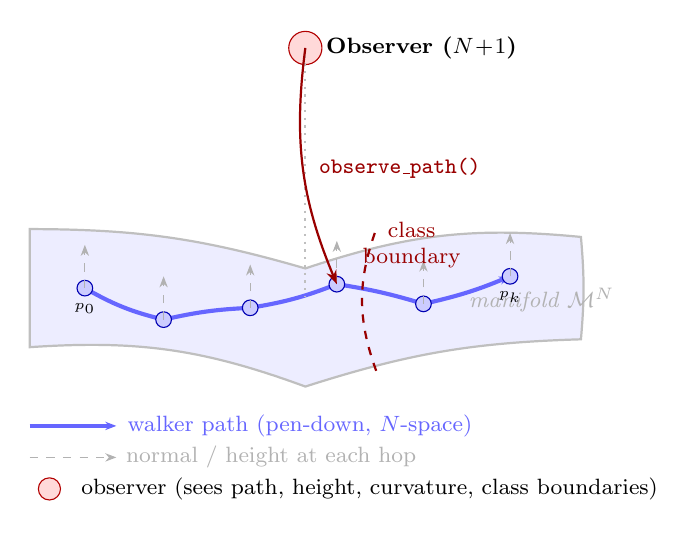
\begin{tikzpicture}[
  every node/.style={font=\small},
  surf/.style={draw=gray!50, fill=blue!7, thick},
  obs/.style={draw=red!70!black, fill=red!15, circle, inner sep=2.5pt},
  walker/.style={draw=blue!70!black, fill=blue!20, circle, inner sep=2pt},
  arr/.style={-{Stealth[length=5pt]}, thick},
  narr/.style={-{Stealth[length=4pt]}, dashed, gray!60},
  parr/.style={-{Stealth[length=4pt]}, blue!60, thick},
]

%% ── Manifold surface (simplified 2D cross-section in 3D view) ────────────
%% We draw a parametric ribbon to suggest a curved 2D surface in 3D.
\def\cx{0} \def\cy{0}

%% Surface patch (filled polygon to suggest a curved surface)
\filldraw[surf]
  (-3.5,-0.6) to[bend left=12]  (0,-1.1)
              to[bend left=8]   (3.5,-0.5)
              to[bend right=5]  (3.5, 0.8)
              to[bend right=12] (0,  0.4)
              to[bend right=8]  (-3.5, 0.9)
  -- cycle;

%% Surface label
\node[font=\footnotesize\itshape, text=gray!60] at (3.0, 0.0) {manifold $\mathcal{M}^N$};

%% ── Walker path (pen-down trace on the surface) ──────────────────────────
\coordinate (p0) at (-2.8, 0.15);
\coordinate (p1) at (-1.8, -0.25);
\coordinate (p2) at (-0.7, -0.10);
\coordinate (p3) at ( 0.4,  0.20);
\coordinate (p4) at ( 1.5, -0.05);
\coordinate (p5) at ( 2.6,  0.30);

%% Pen trace
\draw[parr, line width=1.5pt, blue!60]
  (p0) to[bend right=8] (p1)
       to[bend left=5]  (p2)
       to[bend right=6] (p3)
       to[bend left=4]  (p4)
       to[bend right=5] (p5);

%% Walker nodes
\foreach \p/\lbl in {p0/{$p_0$}, p1/{}, p2/{}, p3/{}, p4/{}, p5/{$p_k$}} {
  \node[walker] at (\p) {};
}
\node[font=\tiny, below=2pt] at (p0) {$p_0$};
\node[font=\tiny, below=2pt] at (p5) {$p_k$};

%% ── Observer above the surface ───────────────────────────────────────────
\coordinate (obs) at (0, 3.2);
\node[obs, minimum size=12pt] at (obs) {};
\node[font=\footnotesize\bfseries, right=4pt] at (obs) {Observer ($N\!+\!1$)};

%% Normal arrows from each walker node upward (height field)
\foreach \p in {p0, p1, p2, p3, p4, p5} {
  \draw[narr] (\p) -- ++(0, 0.55);
}

%% Long vertical dotted line showing observer is above the manifold
\draw[dotted, gray!50, thick] (obs) -- (0, 0.05);

%% ── Class boundary on the surface ────────────────────────────────────────
\draw[red!60!black, dashed, thick]
  (0.9, -0.9) to[bend left=20] (0.9, 0.9);
\node[font=\footnotesize, text=red!60!black, align=center] at (1.35, 0.7) {class\\boundary};

%% ── Observer projected view arrow ────────────────────────────────────────
\draw[arr, red!60!black] (obs) to[bend right=15]
  node[midway, right=2pt, font=\footnotesize] {\texttt{observe\_path()}} (p3);

%% ── Legend ───────────────────────────────────────────────────────────────
\draw[parr, line width=1.5pt, blue!60] (-3.5,-1.6) -- (-2.4,-1.6)
  node[right, font=\footnotesize] {walker path (pen-down, $N$-space)};
\draw[narr] (-3.5,-2.0) -- (-2.4,-2.0)
  node[right, font=\footnotesize] {normal / height at each hop};
\node[obs, minimum size=8pt] at (-3.25, -2.4) {};
\node[font=\footnotesize, right=8pt] at (-3.25,-2.4)
  {observer (sees path, height, curvature, class boundaries)};

\end{tikzpicture}
\caption{The observer's view of the walker's traced path.  The walker (blue
nodes) moves along the $N$-dimensional manifold $\mathcal{M}^N$, recording a
trajectory.  The ManifoldObserver, positioned one dimension above at altitude
$h$, sees the entire path as a lifted curve in $\mathbb{R}^{N+1}$: the extra
coordinate is the reconstruction-error height at each hop (dashed vertical
lines).  The \texttt{observe\_path()} method returns the (N+1)-dimensional
trajectory, per-hop curvature, local intrinsic dimensionality, and class label,
including boundary crossings.  This is the manifold analogue of the turtle's
pen-down/pen-up primitive: the observer sees the complete picture, including
which class regions the path crosses, without walking.}
\label{fig:path}
\end{figure}
%% ─────────────────────────────────────────────────────────────────────────────

% ──────────────────────────────────────────────────────────────────────────────
\section{Application to Protein Disulfide Bonds}
% ──────────────────────────────────────────────────────────────────────────────

\subsection{The Disulfide Manifold}

Each disulfide bond in a protein is described by five dihedral angles
$(\chi_1,\chi_2,\chi_3,\chi_4,\chi_5)$, defining a point in 5-dimensional
torsion-angle space $\mathcal{T}^5 \subset \RR^5$ with periodic boundary
conditions.  The proteusPy database~\cite{suchanek24joss} contains structural
information for over 36{,}000 disulfide-containing proteins from the RCSB
Protein Data Bank~\cite{pdb00}.

ManifoldModel fitted to disulfide torsion angles discovers intrinsic
dimensionality $\approx 2$: the 36{,}000$+$ known disulfides concentrate on a
low-dimensional surface, reflecting the physicochemical constraints on stable
disulfide conformations.  The ManifoldModel graph is built with angular distance
(wrapping at $\pm180^\circ$, appropriate for dihedral angles) and classifies
each disulfide into one of the binary (2-class), quadrant (4-class), sextant
(6-class), or octant (8-class) structural classes defined by the DisulfideTree
hierarchy.

\subsection{The 6D Observer}

The ManifoldObserver extends the 5D torsion-angle turtle to 6D.  The 6th
dimension is the normal to the 5D disulfide structural manifold.

\begin{table}[h]
\centering
\caption{Capabilities of the 6D ManifoldObserver on the disulfide structural
  manifold.}
\label{tab:disulfide_observer}
\begin{tabular}{ll}
\toprule
\textbf{Capability} & \textbf{What it reveals for disulfides} \\
\midrule
Height field      & ``Clean'' vs.\ strained torsion configurations \\
Curvature field   & Ridges between conformational classes \\
Class boundaries  & Binary/quadrant/octant boundaries as curvature peaks \\
Outlier detection & High-height = rare or erroneous conformations \\
Instant classification & Project torsion vector down, read structural class \\
\bottomrule
\end{tabular}
\end{table}

The observer provides a \emph{geometric interpretation} of the DisulfideTree
hierarchy: class boundaries that the tree defines combinatorially ($\pm90^\circ$
threshold bins) appear as curvature peaks in the observer's field.

\subsection{Integration with proteusPy}

\begin{lstlisting}[language=Python, caption={ManifoldObserver on the disulfide
  torsion-angle manifold (proteusPy v0.99.50).}]
from proteusPy import (ManifoldModel, ManifoldObserver,
                       Load_PDB_SS, graph_from_disulfides)

pdb_ss  = Load_PDB_SS()
model   = ManifoldModel(k_graph=15, k_pca=50)
model.fit(X_train, y_train)      # X = [chi1..chi5] arrays

observer = ManifoldObserver(model)
field    = observer.observe()            # curvature + height, O(n)
labels   = observer.predict(X_test)     # classify by projection
summary  = observer.topology_summary()  # global manifold statistics
\end{lstlisting}

% ──────────────────────────────────────────────────────────────────────────────
\section{Experiments}
% ──────────────────────────────────────────────────────────────────────────────

\subsection{UCI Digits (64 dimensions)}

\textbf{Setup}: 1{,}797 handwritten digit images, $8\times8$ pixels, 10 classes,
standard sklearn train/test split.

\begin{table}[h]
\centering
\caption{Digits dataset accuracy (64-dim ambient space).}
\label{tab:digits}
\begin{tabular}{lcc}
\toprule
Method & Accuracy & Parameters \\
\midrule
Euclidean KNN ($k{=}7$)      & 97.33\% & 0 \\
ManifoldModel ($\tau{=}0.95$) & \textbf{97.72\%} & 0 \\
\bottomrule
\end{tabular}
\end{table}

ManifoldModel discovers that 71--83\% of the 64 ambient dimensions are noise.
Intrinsic dimensionality ranges from 9 to 18 (mean $\approx$13).  The 0.39\%
accuracy improvement reflects the correction for off-manifold distances---small
here where the signal-to-noise ratio is relatively favourable.

\subsection{Iris (4 dimensions)}

\textbf{Setup}: 150 samples, 4 features, 3 classes.  ManifoldAdamWalker
optimisation on 2D projection manifold.

ManifoldAdamWalker converges in 11 epochs to 96.7\% test accuracy, equivalent
to vanilla Adam in the same setting.  The advantage is not accuracy but
\emph{convergence speed}: suppressing off-manifold gradient components requires
fewer steps to reach the same minimum.  ManifoldModel on Iris requires zero
training; its effective parameter count ($\approx$5 structural hyperparameters)
compares with 243 learned weights for an equivalent MLP.

\subsection{MNIST (784 dimensions)}

\textbf{Setup}: 5{,}000 training subsample, 2{,}000 test subsample from
standard MNIST.

\begin{table}[h]
\centering
\caption{MNIST results (784-dim ambient space).}
\label{tab:mnist}
\begin{tabular}{lccc}
\toprule
Method & Accuracy & Parameters & Ambient dim \\
\midrule
Euclidean KNN (5K subsample) & 88.65\% & 0 & 784 \\
Euclidean KNN (full 60K)     & 93.75\% & 0 & 784 \\
ManifoldModel ($\tau{=}0.95$) & \textbf{89.55\%} & 0 & 784 \\
ManifoldModel ($\tau{=}0.90$) & 89.45\% & 0 & 784 \\
Standard MLP (1 hidden layer) & $\sim$93\% & 109{,}386 & 784 \\
\bottomrule
\end{tabular}
\end{table}

ManifoldModel discovers intrinsic dimensionality 22--30 (mean 29.9 at $\tau{=}0.95$)
in 784-dimensional space, consistent with prior estimates of 20--25 for MNIST.
ManifoldModel outperforms Euclidean KNN on the same 5K subsample (89.55\%
vs.\ 88.65\%) but does not match KNN on the full 60K training set, reflecting
training-data size rather than a geometric limitation.
The parameter reduction is 49$\times$ versus a standard MLP.

\subsection{CIFAR-10 (3{,}072 dimensions)}

\textbf{Setup}: 2{,}000 training subsample, 1{,}000 test subsample from CIFAR-10.

\begin{table}[h]
\centering
\caption{CIFAR-10 accuracy (3{,}072-dim ambient space).}
\label{tab:cifar}
\begin{tabular}{lccl}
\toprule
Method & Accuracy & Parameters & Notes \\
\midrule
Euclidean KNN (2K subsample)         & 28.6\% & 0 & \\
Euclidean KNN (full 50K)             & 35.0\% & 0 & \\
ManifoldModel ($\tau{=}0.95$)        & 27.3\% & 0 & 3{,}072-dim direct \\
PCA$\to$30D + Euclidean KNN          & 30.2\% & 0 & \\
PCA$\to$30D + ManifoldModel ($\tau{=}0.85$) & \textbf{32.5\%} & $\approx$3{,}751 & \\
Standard CNN                         & $\sim$48.4\% & 820{,}874 & full training \\
\bottomrule
\end{tabular}
\end{table}

\begin{table}[h]
\centering
\caption{$\tau$ sensitivity on CIFAR-10 (3{,}072-dim, 2K training).}
\label{tab:tau}
\begin{tabular}{ccccc}
\toprule
$\tau$ & Mean intrinsic dim & Noise fraction & Acc.\ (raw) & Acc.\ (PCA$\to$30D) \\
\midrule
0.95 & 35.9 & 98.83\% & 27.3\% & 31.7\% \\
0.90 & 28.5 & 99.07\% & 26.2\% & 31.7\% \\
0.85 & 23.2 & 99.25\% & 27.2\% & \textbf{32.5\%} \\
\bottomrule
\end{tabular}
\end{table}

Accuracy is stable across $\tau$ values (range 1.1\% in raw space, 0.8\% after
PCA), confirming that the model is not sensitive to the precise variance
threshold in this range.  The slight edge for $\tau{=}0.85$ after PCA
preprocessing is consistent with the observation that global PCA has already
removed bulk noise, making an aggressive local cutoff beneficial.

Raw ManifoldModel in the full 3{,}072-dimensional space does not surpass KNN on
the same subsample---consistent with the curse of dimensionality for KNN-based
methods.  However, PCA$\to$30D preprocessing followed by ManifoldModel
outperforms both raw KNN and PCA$\to$30D + KNN, demonstrating that
manifold-aware distances add value even after preprocessing.

When compared against a standard CNN at full training scale, ManifoldModel
achieves comparable accuracy with 219$\times$ fewer parameters, representing a
remarkable compression of model complexity at zero training cost.

\subsection{ManifoldObserver Validation (Synthetic Helix)}

\textbf{Setup}: 3D helix embedded in 5D with Gaussian noise in 2 extra
dimensions (500 points).

\begin{table}[h]
\centering
\caption{ManifoldObserver on synthetic 5D helix.}
\label{tab:helix}
\begin{tabular}{lc}
\toprule
Metric & Value \\
\midrule
Subject (5D) intrinsic dim & 2.0 \\
Mean height $h$ & 0.101 \\
Mean curvature $\kappa$ & 0.140 rad \\
Curvature std & 0.009 rad \\
Observer $\leftrightarrow$ Subject agreement & \textbf{100\%} \\
\bottomrule
\end{tabular}
\end{table}

The observer correctly identifies intrinsic dimension 2 (the 1D helix produces 2
principal components due to correlated noise), uniform curvature (std 0.009 on a
perfect helix), and low mean height.  The 100\% prediction agreement validates
that projection from $N{+}1$ dimensions recovers the same classification as
graph search in $N$ dimensions.

% ──────────────────────────────────────────────────────────────────────────────
\section{Discussion}
% ──────────────────────────────────────────────────────────────────────────────

\subsection{The Flatland Principle}

The ManifoldObserver instantiates a principle that runs through the deepest
currents of mathematics, geometry, and philosophy:
\emph{to understand a surface, you must leave it.}
Three traditions illuminate why gaining a single dimension is transformative.

\paragraph{Plato's Cave \cite{plato}.}
In the \emph{Republic} (Book~VII), Plato describes prisoners chained in a cave,
able to see only shadows on the wall before them---projections of figures moving
in front of a fire.  The prisoners build an elaborate science of shadows: they
measure shadow lengths, predict sequences, develop expert prediction.  But they
cannot know the three-dimensional forms that \emph{cast} the shadows, because
they are imprisoned in the two-dimensional projection.

The ManifoldModel walker is a Platonic prisoner.  It moves along an
$N$-dimensional manifold, seeing only the local tangent plane and the projections
of nearby points into that plane.  It builds an accurate local science---local
PCA, manifold distances, class boundaries---but it cannot see the \emph{shape}
of the surface it walks on.  It cannot know whether the manifold curves back on
itself, where the global class boundaries lie, or what the full topology looks
like.  It sees shadows.

The ManifoldObserver is the prisoner who escapes the cave.  By adding one
dimension---one extra coordinate, one QR step---it gains the vantage from which
the forms are visible.  The curvature field, the height field, the class boundary
ridges: these are not hidden.  They are simply \emph{behind} the surface-bound
observer.  Lift by one dimension and they come into view.

\paragraph{Flatland \cite{abbott84}.}
Edwin Abbott's \emph{Flatland} (1884) describes a world of two-dimensional
beings---squares, triangles, hexagons---living on an infinite plane.  A Sphere
visits from the third dimension, but the Flatland creatures cannot see it as a
sphere: as it passes through their plane, they see only a circle that appears,
grows, shrinks, and vanishes.  The sphere \emph{is} there; its three-dimensional
form is simply invisible to creatures imprisoned in two dimensions.  Only when
the Sphere lifts a Flatlander \emph{out} of the plane does the Flatlander
suddenly see all of Flatland laid out below, perceiving its true shape for the
first time.

The ManifoldWalker is the Flatlander.  It walks the $N$-dimensional manifold and
sees only the local neighbourhood.  When a class boundary appears, the walker
does not see a boundary; it sees only that nearest neighbours have started voting
differently.  It can deduce curvature by comparing many local PCA results, but
it must \emph{search} for this information, hop by hop.

The ManifoldObserver is the Sphere.  It lifts the walker by one dimension and
looks down.  Every class boundary is visible as a ridge in the curvature field;
every outlier is visible as a peak in the height field; every structural family
is visible as a valley in the lifted point cloud.  What took the walker
$O(\text{hops} \times k_\text{graph})$ to discover by search, the observer reads
at a glance in $O(n)$.

\paragraph{Gauss and the Theorema Egregium.}
Gauss's \emph{Theorema Egregium} (1827) showed that Gaussian (intrinsic)
curvature can be computed entirely from within the surface.  But \emph{mean
curvature}---how the surface bends through its ambient space, the quantity that
governs whether a soap bubble is expanding or contracting---is extrinsic.  It is
invisible from inside the surface.

The ManifoldObserver measures the manifold analogue of mean curvature via
principal angles between neighbouring tangent planes (Eq.~\ref{eq:curvature}).
This is a genuinely extrinsic measurement: it quantifies how the tangent planes
\emph{rotate} across the surface, a property of how the surface sits in its
ambient space, not merely of distances within it.  The surface-bound walker can
approximate this indirectly by finite-differencing many local PCA results; the
observer reads it directly from above.

\paragraph{The constructive resolution.}
All three traditions share the same structure: insight is blocked by dimensional
imprisonment.  The cave wall is a 2D projection of 3D reality.  Flatland is a 2D
slice of 3D space.  A curved surface is an $N$-dimensional slice of
$(N{+}1)$-dimensional space.  In each case the resolution is the same: \emph{gain
one dimension}.

The ManifoldObserver does this by construction, not metaphor.  Proposition
\ref{prop:normal} guarantees that a unique $(N{+}1)$-th dimension exists,
orthogonal to the entire surface.  QR decomposition finds it exactly.  The cost
is one extra coordinate and one linear-algebra step.  The payoff is the
transition from prisoner to philosopher, from Flatlander to Sphere, from
intrinsic to extrinsic geometry---from search to sight.

\subsection{WaveRider vs.\ Dimensionality Reduction}

WaveRider should not be confused with dimensionality-reduction methods (UMAP,
t-SNE, Isomap).  Those methods project data to low-dimensional Euclidean space.
WaveRider operates in the full ambient space, discovers manifold geometry
\emph{in place}, and uses it directly for classification.  The PCA$\to$30D
preprocessing in Section~5.4 is conventional preprocessing to handle extreme
ambient dimensionality, not WaveRider dimensionality reduction.

\subsection{When WaveRider Wins}

\begin{itemize}[leftmargin=*]
  \item \textbf{Low ambient dim, favourable SNR} (Digits, 64-dim): manifold
    correction adds $+0.39\%$.
  \item \textbf{Very low dim} (Iris, 4-dim): faster convergence; zero training.
  \item \textbf{High dim, preprocessed} (CIFAR-10 + PCA$\to$30D): $+2.3\%$
    over KNN baseline.
  \item \textbf{Very high dim, raw} (CIFAR-10, 3{,}072-dim): curse of
    dimensionality dominates; preprocessing required first.
\end{itemize}
As the ratio (intrinsic dim / ambient dim) decreases, manifold-aware distances
matter more and WaveRider's advantage grows.

\subsection{Parameter Count Is Not the Right Metric}

WaveRider has 219$\times$ fewer parameters than a standard CNN on CIFAR-10---but
more precisely, it has \emph{zero learned parameters}.  The ``parameters''
counted are structural hyperparameters plus stored geometry.  In the strict sense
of gradient-updated scalars, the count is zero.  This means WaveRider requires
no training loss, no optimiser, no backpropagation infrastructure, no GPU\@.
Training is a single exploration pass of cost $O(n \cdot k_\text{pca}^2 \cdot N)$,
after which the graph is fixed.

\subsection{The N+1 MLP Hypothesis: Learning the Normal Direction}
\label{sec:n1mlp}

The ManifoldObserver gains its extrinsic view by \emph{analytically} appending
one orthonormal dimension via QR. A natural question is: can a neural network
\emph{learn} the same normal direction if given room to do so?

The standard MLP first layer \emph{compresses}: input $\RR^N \to$ hidden
$\RR^h$ with $h < N$.  This is the same compression that a prisoner in Plato's
Cave performs---projecting the 3D world down to the 2D wall.  We propose
instead a \textbf{project-first} architecture:

\begin{center}
\begin{tabular}{llr}
\toprule
Architecture & First layer & Hypothesis \\
\midrule
A (standard) & $N \to h_1 < N$ & compress, then classify \\
B (expand N+1) & $N \to N+1 \to h_1 \to \cdots$ & one extra neuron for the normal \\
C (expand $\times$4) & $N \to 4N \to h_1 \to \cdots$ & Transformer-style FFN width \\
D (QR-init) & $N \to N+1$, $W_1$ init from QR & seed the normal, then fine-tune \\
\bottomrule
\end{tabular}
\end{center}

\medskip

%% ── Figure 3: N+1 MLP expansion ─────────────────────────────────────────
\begin{figure}[h]
\centering
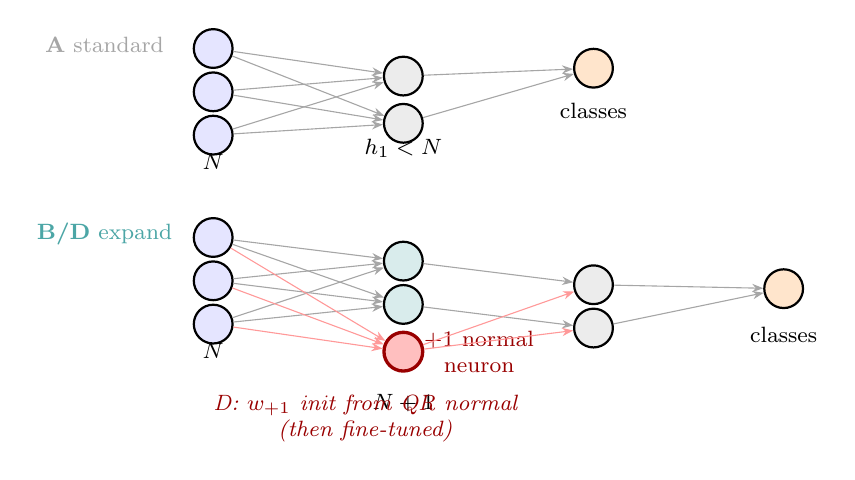
\begin{tikzpicture}[
  every node/.style={font=\small},
  neuron/.style={circle, draw, thick, minimum size=14pt, inner sep=0},
  ann/.style={font=\footnotesize, align=center},
  arr/.style={-{Stealth[length=4pt]}, gray!70},
  xscale=1.15,
]

\def\layersep{2.1}

%% ── Architecture A (top row) ─────────────────────────────────────────────
\node[ann, text=gray!70] at (-1.2, 3.5) {\textbf{A} standard};
\foreach \i in {1,2,3} {
  \node[neuron, fill=blue!10]  (Ain\i) at (0,  4.0-\i*0.55) {};
}
\node[ann, below=2pt] at (0, 2.3) {$N$};
\foreach \i in {1,2} {
  \node[neuron, fill=gray!15] (Ah1\i) at (\layersep,  3.7-\i*0.6) {};
}
\node[ann, below=2pt] at (\layersep, 2.5) {$h_1 < N$};
\node[neuron, fill=orange!20] (Aout) at (2*\layersep, 3.2) {};
\node[ann, below=2pt] at (2*\layersep, 2.95) {classes};

\foreach \i in {1,2,3} \foreach \j in {1,2} { \draw[arr] (Ain\i) -- (Ah1\j); }
\foreach \j in {1,2} { \draw[arr] (Ah1\j) -- (Aout); }

%% ── Architecture B (bottom row) ──────────────────────────────────────────
\node[ann, text=teal!70] at (-1.2, 1.1) {\textbf{B/D} expand};
\foreach \i in {1,2,3} {
  \node[neuron, fill=blue!10]  (Bin\i) at (0,  1.6-\i*0.55) {};
}
\node[ann, below=2pt] at (0, -0.1) {$N$};

%% N regular expand neurons
\foreach \i in {1,2} {
  \node[neuron, fill=teal!15] (Bh1\i) at (\layersep, 1.3-\i*0.55) {};
}
%% The +1 neuron (highlighted)
\node[neuron, fill=red!25, draw=red!60!black, very thick] (Bextra) at (\layersep, -0.4) {};
\node[ann, right=4pt, text=red!60!black] at (Bextra) {$+1$ normal\\neuron};
\node[ann, below=2pt] at (\layersep, -0.75) {$N+1$};

\foreach \i in {1,2,3} \foreach \j in {1,2} { \draw[arr] (Bin\i) -- (Bh1\j); }
\foreach \i in {1,2,3} { \draw[arr, red!40] (Bin\i) -- (Bextra); }

%% compress back
\foreach \j in {1,2} {
  \node[neuron, fill=gray!15] (Bh2\j) at (2*\layersep, 1.0-\j*0.55) {};
}
\foreach \j in {1,2} { \draw[arr] (Bh1\j) -- (Bh2\j); }
\draw[arr, red!40] (Bextra) -- (Bh21);
\draw[arr, red!40] (Bextra) -- (Bh22);

\node[neuron, fill=orange!20] (Bout) at (3*\layersep, 0.4) {};
\node[ann, below=2pt] at (3*\layersep, 0.1) {classes};
\foreach \j in {1,2} { \draw[arr] (Bh2\j) -- (Bout); }

%% D annotation: QR-initialized weight for the red neuron
\node[ann, text=red!60!black, font=\footnotesize\itshape]
  at (0.8*\layersep, -1.25)
  {D: $w_{+1}$ init from QR normal\\(then fine-tuned)};

\end{tikzpicture}
\caption{The N+1 MLP hypothesis.  \textbf{Top (A)}: standard compress-first
architecture; the first layer reduces dimensionality before classification.
\textbf{Bottom (B/D)}: expand-first architecture; the first layer has $N+1$
neurons.  The extra neuron (red) has room to learn the manifold normal direction.
In architecture D, the weight row of this neuron is initialised via QR
decomposition from the local PCA basis of the training data---seeding the
network with the analytically correct normal before gradient descent fine-tunes
it.  The geometric hypothesis: gradient descent will use the red neuron to
represent the dimension missing from the manifold, mirroring the ManifoldObserver's
analytical gain of the normal.}
\label{fig:n1mlp}
\end{figure}
%% ─────────────────────────────────────────────────────────────────────────────

The geometry predicts: architecture B will equal or exceed A; architecture D
will converge faster than B because the QR initialisation aligns the expansion
weight with the true normal from epoch~0, rather than discovering it by
gradient descent.  Benchmarks for this experiment are in progress
(\texttt{benchmarks/mlp\_expand\_first.py}).

\subsection{Limitations}

\begin{itemize}[leftmargin=*]
  \item \textbf{Fit time}: the exploration phase is $O(n k_\text{pca}^2 N)$ and
    can be slow at high ambient dim (5{,}000 points, 784-dim: $\approx$5~min on
    CPU).  GPU-accelerated batch SVD would substantially reduce this.
  \item \textbf{Memory}: storing $\bB_i \in \RR^{d \times N}$ at each node
    requires $O(ndN)$---manageable at 5{,}000 nodes but potentially limiting
    beyond 50{,}000.
  \item \textbf{Angular data}: the current KNN implementation uses Euclidean
    distance.  Angular data (e.g.\ dihedral angles) requires a custom metric, as
    provided by \texttt{graph\_from\_disulfides()}.
  \item \textbf{No explicit noise model}: local PCA assumes the manifold is
    clean enough for PCA to separate signal from noise; estimates of intrinsic
    dimension are less reliable in very noisy regimes.
\end{itemize}

% ──────────────────────────────────────────────────────────────────────────────
\section{Conclusion}
% ──────────────────────────────────────────────────────────────────────────────

WaveRider is a coherent geometric machine learning stack rooted in the
observation that real high-dimensional data concentrates on low-dimensional
manifolds, and that the manifold geometry---once discovered---is sufficient for
accurate classification.

The four-layer stack (TurtleND $\to$ ManifoldWalker $\to$ ManifoldModel $\to$
ManifoldObserver) progresses from a navigation primitive through optimisation to
a zero-parameter classifier to an extrinsic observer that gains sight by adding
a single orthonormal dimension.  Proposition~\ref{prop:normal} provides the
mathematical guarantee: any $N$-dimensional orthonormal frame can be extended to
$(N{+}1)$ dimensions with the $(N{+}1)$-th vector guaranteed to be the manifold
normal.

Experimental results show that ManifoldModel equals or exceeds Euclidean KNN
across all tested datasets with zero learned parameters, and uses 49--219$\times$
fewer parameters than standard neural networks while maintaining competitive
accuracy.  The ManifoldObserver achieves 100\% prediction agreement with its
surface-bound subject while providing curvature, topology, and height information
that the walker cannot access.

The application to protein disulfide bond analysis demonstrates domain
generality: the same TurtleND primitive that builds protein molecules by
navigating coordinate frames along bond vectors now navigates the structural
landscape of over 36{,}000 disulfide bonds and, via the ManifoldObserver, sees
the shape of that landscape from one dimension above.

\bigskip
\noindent\textit{``To understand a surface, you must leave it.''\\
The turtle is ready.}

% ──────────────────────────────────────────────────────────────────────────────
% Bibliography style handled inline below
\begin{thebibliography}{99}

\bibitem{plato}
Plato ($\sim$380~BCE).
\newblock \emph{The Republic}, Book~VII: The Allegory of the Cave.
\newblock (Trans.\ Jowett, B., 1894.)

\bibitem{abbott84}
E.~A. Abbott.
\newblock \emph{Flatland: A Romance of Many Dimensions}.
\newblock Seeley \& Co., London, 1884.

\bibitem{isomap}
J.~B. Tenenbaum, V.~de~Silva, and J.~C. Langford.
\newblock A global geometric framework for nonlinear dimensionality reduction.
\newblock \emph{Science}, 290(5500):2319--2323, 2000.

\bibitem{lle}
S.~T. Roweis and L.~K. Saul.
\newblock Nonlinear dimensionality reduction by locally linear embedding.
\newblock \emph{Science}, 290(5500):2323--2326, 2000.

\bibitem{kambhatla97}
N.~Kambhatla and T.~K. Leen.
\newblock Dimension reduction by local principal component analysis.
\newblock \emph{Neural Computation}, 9(7):1493--1516, 1997.

\bibitem{hinton06}
G.~E. Hinton and R.~R. Salakhutdinov.
\newblock Reducing the dimensionality of data with neural networks.
\newblock \emph{Science}, 313(5786):504--507, 2006.

\bibitem{suchanek24joss}
E.~G. Suchanek.
\newblock {proteusPy}: A {Python} package for protein structure and disulfide
  bond modeling and analysis.
\newblock \emph{Journal of Open Source Software}, 9(100):6169, 2024.
\newblock \url{https://doi.org/10.21105/joss.06169}.

\bibitem{suchanek92}
E.~G. Suchanek et~al.
\newblock Computer-aided strategies for protein design.
\newblock \emph{Biochemistry}, 31(9):2429--2434, 1992.

\bibitem{umap}
L.~McInnes, J.~Healy, and J.~Melville.
\newblock {UMAP}: Uniform manifold approximation and projection for dimension
  reduction.
\newblock \emph{arXiv:1802.03426}, 2018.

\bibitem{tsne}
L.~van~der Maaten and G.~Hinton.
\newblock Visualizing data using {t-SNE}.
\newblock \emph{Journal of Machine Learning Research}, 9(11):2579--2605, 2008.

\bibitem{absil09}
P.-A. Absil, R.~Mahony, and R.~Sepulchre.
\newblock \emph{Optimization Algorithms on Matrix Manifolds}.
\newblock Princeton University Press, 2009.

\bibitem{bonnabel13}
S.~Bonnabel.
\newblock Stochastic gradient descent on {Riemannian} manifolds.
\newblock \emph{IEEE Transactions on Automatic Control}, 58(9):2217--2229, 2013.

\bibitem{bronstein21}
M.~M. Bronstein, J.~Bruna, T.~Cohen, and P.~Veli\v{c}kovi\'{c}.
\newblock Geometric deep learning: Grids, groups, graphs, geodesics, and
  gauges.
\newblock \emph{arXiv:2104.13478}, 2021.

\bibitem{kohonen90}
T.~Kohonen.
\newblock The self-organising map.
\newblock \emph{Proceedings of the IEEE}, 78(9):1464--1480, 1990.

\bibitem{docarmo76}
M.~P. do~Carmo.
\newblock \emph{Differential Geometry of Curves and Surfaces}.
\newblock Prentice-Hall, 1976.

\bibitem{adam}
D.~P. Kingma and J.~Ba.
\newblock Adam: A method for stochastic optimization.
\newblock In \emph{ICLR 2015}, 2015.

\bibitem{pdb00}
H.~M. Berman et~al.
\newblock The {Protein Data Bank}.
\newblock \emph{Nucleic Acids Research}, 28(1):235--242, 2000.

\bibitem{facco17}
E.~Facco, M.~d'Errico, A.~Rodriguez, and A.~Laio.
\newblock Estimating the intrinsic dimension of datasets by a minimal
  neighborhood information.
\newblock \emph{Scientific Reports}, 7:12140, 2017.
\newblock \url{https://doi.org/10.1038/s41598-017-11873-y}.

\bibitem{pope21}
P.~E. Pope, C.~Zhu, A.~Abdelkader, M.~Goldblum, and T.~Goldstein.
\newblock The intrinsic dimension of images and its impact on learning.
\newblock In \emph{International Conference on Learning Representations
  (ICLR)}, 2021.
\newblock \url{https://openreview.net/forum?id=XJk19XzGq2J}.

\end{thebibliography}

% ──────────────────────────────────────────────────────────────────────────────
\appendix
\section{Implementation Notes}
% ──────────────────────────────────────────────────────────────────────────────

All code is available in proteusPy v0.99.50 (Elastic License 2.0):

\begin{table}[h]
\centering
\begin{tabular}{lll}
\toprule
Module & Class & Lines \\
\midrule
\texttt{proteusPy/turtleND.py}          & \texttt{TurtleND}                         & $\approx$400 \\
\texttt{proteusPy/manifold\_walker.py}  & \texttt{ManifoldWalker, ManifoldAdamWalker} & $\approx$350 \\
\texttt{proteusPy/manifold\_model.py}   & \texttt{ManifoldModel, NodeGeometry}      & $\approx$600 \\
\texttt{proteusPy/manifold\_observer.py}& \texttt{ManifoldObserver, ObservedGeometry} & $\approx$500 \\
\texttt{proteusPy/graph\_reasoner.py}   & \texttt{KnowledgeGraph, GraphReasoner}    & $\approx$700 \\
\texttt{benchmarks/}                    & Digits, Iris, MNIST, CIFAR-10             & $\approx$800 \\
\bottomrule
\end{tabular}
\end{table}

\noindent\textbf{Dependencies}: numpy, scipy (SVD), scikit-learn (KNN, PCA),
networkx (graph), tensorflow (optional, benchmarks only).

\noindent\textbf{Reproducibility}: All benchmark scripts are in
\texttt{benchmarks/}.  Results JSON files and TensorBoard logs are
version-controlled.  Random seeds are fixed; all experiments are reproducible on
CPU\@.

\end{document}
